\chapter{Preliminaries}
\label{chapter:preliminaries}

In this chapter, we define the concepts used throughout the dissertation.
First,
in Section\:\ref{events-enactments},
we introduce an event stream model
for sequences of events, ordered by timestamps and carrying data,
called ``enactments''.
In Section\:\ref{rule-language}
we introduce a language
for specifying constraints on enactments,
called ``business process rules''
or ``rules'' for short.
Rules use Datalog syntax \cite{ceri1989you},
with the addition of
(i) syntax for separating an event's data from its timestamp,
(ii) inequality predicates and arithmetic on event timestamps,
and
(iii) existential variables in the rule head,
and (iv) multiple atoms in the rule head.
Our interpretation of rules differs from Datalog in that
we treat rules as constraints,
not as programs that generate events.
We define the semantics of rule satisfaction and violation,
then
define what it means to detect violations at the earliest possible time.
In Section\:\ref{sec:motiv},
we illustrate the basic concepts
of our approach to violation detection
with an example.

\section{Events and Workflow Enactments}
\label{events-enactments}

To describe events,
we assume the following pairwise-disjoint, infinite sets:
\begin{itemize}
    \item $\mathcal{E}$ of event names, 
      typically single words in typewriter font with a capitalized first letter,
      e.g., {\tt Request}, {\tt Payment}, ...
    \item $\mathcal{A}$ of attribute names,
      typically single, italicized, lowercase words,
      e.g., {\it user}, ...
    \item $\ID$ of {\em enactment identifiers}, or simply {\eid}'s,
    to identify the enactment to which an event belongs,
    \item A data domain $\Dom$ of uninterpreted constants,
	    with the equality ($=$) and non-equality predicate ($\neq$), and
    % \item {\bf Isaac: A numeric domain for aggregation}, and
      %We use the natural numbers $\mathcal{N}$.
    \item Discrete timestamps. Without loss of generality,
      we use the natural numbers $\mathbb{N}$ as timestamps,
      with the standard addition operation ($+$)
      and equality, non-equality, and inequalities predicates ($=$, $\neq$, $<$, $\dots$) 
      as well as the integers $\mathbb{Z}$ for related technical development.
\end{itemize}

We study early violation detection
in the context of monitoring
event streams generated by enactments of workflows.
In a workflow, activities are atomic units of work,
e.g., a {\Request} arrives and is processed.
We treat the completion of an activity
as an event with no duration.

{\it Definition}.
An {\em event type} $E(a_1,\dots,a_n)$, 
where $n\geq 0$,
has an event name $E$ from $\mathcal{E}$
and a fixed set of {\em attributes} $a_1$, $\dots$, $a_n$, each from $\mathcal{A}$.
An event type is {\em dataless} if it has no attributes, i.e., $n=0$.
An {\em event (instance)} of an event type $E(a_1,...,a_n)$
is a named tuple $E(c_1,...,c_n)@t$ where
$c_i$ is a value from $\Dom$
for each attribute $a_i$
and $t$ is a timestamp from $\mathbb{N}$.

For a given workflow,
its schema is a set of event types
for its component activities,
each with the activity's name and data attributes.
We assume that the schema is fixed
and known to the monitor {\em a priori}.
Events are generated by the completion of the activities in a workflow,
so each event carries with an enactment identifier from $\ID$.

{\it Definition}.
An {\em enactment} of a workflow
is a finite set $\eta$ of events,
such that
(i) each event has the same enactment {\sc id},
(ii) $\eta$ has exactly one special event of type {\Start}
that marks its beginning
and at most one {\End} event
that marks its completion,
(iii)
the timestamp of the {\Start} event is
less than that of all other events in $\eta$, and
(iv)
the timestamp of the {\End} event, if it occurs,
is greater than that of all other events in $\eta$.

Workflow enactments
are updated by the completion of new events,
grouped by timestamp:
a {\em batch} for an enactment $\eta$
is a finite set $\Delta$ of events such that
(i) all events in $\Delta$ have the same timestamp,
denoted as $\tmsp_\Delta$,
greater than the timestamps of all events in $\eta$,
(ii) for each event $e$ in $\Delta$,
the {\sc id} of $e$ is the {\sc id} of $\eta$,
(iii) $\Delta$ has a {\Start} event or $\eta$ has a {\Start} event,
but not both, and
(vi) if an {\End} event is in $\eta$,
no events are in $\Delta$.

% Fig.\:\ref{fig:example_state} shows
% events from two enactments
% of the workflow in the IaaS example.
% Suppose that
% at time $10$
% exactly two events happened,
% $e_1{:}\Rn{Approval}(\pi_{_1\!},\allowbreak[\An{Alice}], 10)$
% and
% $e_2{:}\Rn{Approval}(\pi_{_2\!},\allowbreak[\An{Bob}], 10)$.
% Then 
% $\{e_1\}$ is a batch
% for $\pi_{_1\!}$,
% $\{e_2\}$ a batch
% for $\pi_{_2\!}$.

\section{Rules}
\label{rule-language}

We express constraints in a language first introduced in \cite{mackey2022rule},
named here {\em (business process) rules},
or simply {\em rules}.
The rule language
It uses a Datalog-like syntax,
but unlike Datalog,
the rule syntax separates an event's data from its timestamp,
allows multiple atoms and existential variables in the rule head,
and gap atoms with inequalities on time variables.
First, we provide the rule syntax,
then we define what it means for an enactment
to satisfy or violate a rule or set of rules.

We start with atomic formulas.
We use the existing sets from the previous section
and define the following infinite set,
disjoint from the others:
$\mathcal{V}$ of {\em variables},
typically lowercase letters, 
e.g., $a, b, c, x, y, z, \dots$. 
We use the notation $\bar{x}$ to denote vectors of variables.
An {\em event atom}
is an expression ``$A(v_1,...,v_n)@x$''
where $A(\att_1,...,\att_n)$ is an event type,
$v_1,...,v_n,x$ are variables in $\mathcal{V}$
or constants in $\Dom$ or $\mathbb{N}$.
If $x$ is a variable,
$x$ is a {\it timestamp variable}.
Additionally, constant addition is allowed on timestamps,
i.e., $v+c$ is a valid term for a timestamp,
with variable $v$ and constant $c\in\mathbb{Z}$.
When an event type $E$ is dataless,
the event atom is written as $E@x$ instead of $E()@x$.
A {\em gap atom} (inspired by \cite{Re93}) is
an expression ``$x{\pm}\epsilon \tight\theta y$''
% or ``$x{-}b \tight\theta y$'',
where $x,y$ are timestamp variables,
$\epsilon$ (the gap) is a constant in $\mathbb{Z}$,
and
$\theta\tight\in\{<,\leq,\allowbreak\geq,>,=\}$
is an equality or inequality predicate.
The set of variables in a set of atoms $\varphi$
is denoted $var(\varphi)$.
An event atom $E(\dots)@x$ expresses
that an instance of $E$ happens at time $x$,
e.g.,\ $\Request(\mbox{\em u})@x$ denotes a $\Request$
for some user $u$ at time $x$.

A gap atom $x \tight{\leq_n} y$ means $x \tight+ n \tight\leq y$,
i.e., $x\tight+n$ no later than time $y$.
Similarly,
$x \tight{\geq_n} y$ means $x \tight+ n \tight\geq y$,
i.e., $x\tight+n$ is no earlier than time $y$.
Some gap atoms do not impose an ordering:
when $n\tight>0$, $x \tight{\geq_n} y$ indicates
$y$ is at most $n$ time units after $x$ and potentially
simultaneous with or before $x$.
Note that for each positive $n\tight\in\N$,
$x \tight{\geq_n} y$ does not imply $x \tight\geq y$.

\begin{examp}
Consider the set of atoms
``\Request(\mbox{\em u})$@x$, \Schedule(\mbox{\em u})$@y$,
$x \tight{\leq_{4}} y, x\tight{\geq_{6}} y$''.
Intuitively, it selects
a \Request\ event and a \Schedule\ event
from the same enactment
by the same user $\mbox{\em u}$
that follows the \Request\ by four, five, or six timestamps.
\end{examp}

{\it Definition}.
A {\em rule} is an expression
``$\varphi\tight\to\psi$''
where the {\em body} $\varphi$
and the {\em head} $\psi$
are finite, possibly empty,
sets of event and gap atoms
such that
the body is {\em closed}:
each variable in $\varphi$
occurs in some event atom in $\varphi$, and
the head is closed with respect to the head and body:
each variable in $\psi$
occurs in some event atom in $\varphi\tight\cup\psi$.
Furthermore,
if the body of a rule $\varphi\rightarrow\psi$
has no atoms,
the rule is written $\true\rightarrow\psi$,
with the natural semantics.
  
\begin{examp}\label{ex:rule}
  The following rule $r_0$ requires
  for each pair of {\Request} and subsequent {\Schedule} events
  from the same user $u$,
  there is a subsequent {\Payment} no later than three days after the {\Schedule}
  by that user:

  \begin{center}
  $r_{0}:\ \Request(\mbox{\em u})@x, \Schedule@y, x\leq_{0}y
  \rightarrow
  \Payment(\mbox{\em u})@z, y\leq_{0} z, y\geq_{3} z$
  \end{center}
  \vspace{-2.5em}
\end{examp}

Rule satisfaction is defined
with respect to ``assignments''
from values in the event stream,
which come from $\Dom$ and $\N$,
to rule variables.
An {\em assignment} is a mapping 
from rule variables to values in $\Dom\cup\N$.
An assignment is {\em complete} if it is a total mapping
for the variables in a given set of atoms.
An assignment $\beta$ {\em extends} an assignment $\alpha$
if $\alpha\subseteq\beta$.
An enactment $\eta$ {\em satisfies}
an event atom $A(v_1,...,v_n)@x$
for the event $A(\att_1, ..., \att_n)$
with an assignment $\mu$
if
(1) $\mu$ is defined for $v_1,...,v_n,x$, and
% (2) $A(\eta.\eid,\{\att_1\mapsto\mu(v_1),\dots,
% \att_n\mapsto\mu(v_n)\}, \mu(x))$
(2) $A(\mu(v_1),\dots,\mu(v_n))@\mu(x)$
is an event in $\eta$.
%and $\xi$ is the {\eid} of the enactment $\eta$.
{\em Satisfaction} for gap atoms is defined naturally.
A set of atoms is called a {\em constraint}:
two constraints $\phi$ and $\phi'$ are {\em equivalent} if
for each enactment $\eta$ and assignment $\sigma$,
$\eta\models\phi[\sigma]$ iff $\eta\models\phi'[\sigma]$.
An enactment $\eta$ {\em satisfies}
a set of atoms $\phi$
with an assignment $\mu$
if $\eta$ satisfies every atom in $\phi$ with $\mu$.

% \begin{examp}\label{ex:semantics}
%   As shown in Fig.\:\ref{fig:example_deadline_minimum},
%   the assignment
%   $\mu_{10}$
%   satisfies $\varphi$.
%   Then,
%   to satisfy the rule w.r.t. $\mu_{10}$,
%   there must be an assignment extending $\mu$
%   that satisfies $\psi$;
%   i.e.,
%   two events
%   $\Rn{Payment}(\pi_{_1\!},[\An{Alice},\allowbreak\An{a4}], t_{1\!})$
%   and
%   $\Rn{Launch}(\pi_{_1\!},[\An{Alice},\An{a4}], t_{2\!})$
%   with $6{\leq} t_1{\leq} 6{+}3{=}9$,
%   $8{\leq} t_2{\leq} 8{+}7{=}15$,
%   and
%   $t_2{\leq}t_1{+}4$
%   must happen.
% \end{examp}

We can now define the central notions of
how an enactment satisfies or violates
a rule or a set of rules.
Informally, this is done by
matching assignments
for the body variables
with those for the head variables.
Let $r:\:{\varphi}\tight\rightarrow{\psi}$ be a rule
and
$\eta$ an enactment.
Then, $\eta$ {\em satisfies} $\varphi\tight\to\psi$
if for every assignment $\mu$ such that
$\eta$ satisfies $\varphi$ with $\mu$,
there is an assignment $\beta$ that extends $\mu$
such that $\eta$ satisfies $\psi$ with $\beta$.
Alternatively,
$\eta$ has a {\em potential violation}
of a rule ${\varphi}\tight\rightarrow{\psi}$
with witness $\mu$
if
$\eta$ satisfies $\varphi$ with $\mu$ and
there is no assignment $\beta$ that extends $\mu$
such that $\eta$ satisfies $\psi$ with $\beta$.

%
% An assignment $\mu$ is a {\em potential violation}
% of a rule $r{:}\:{\varphi}\tight\rightarrow{\psi}$
% for an enactment $\eta$
% if
% $\eta$ satisfies $\varphi$ with $\mu$ and
% there is no assignment $\beta$ that extends $\mu$
% such that $\eta$ satisfies $\psi$ with $\beta$.
%
A potential violation becomes inevitable, or permanent,
when it cannot be resolved in any possible future
of the current enactment.
The enactment $\eta$ has a {\em (permanent), violation}
of a rule $r$ 
with a witness $\mu$
if it has a potential violation with $\mu$ and
for every sequence $\seq{\Delta}{n}$ of batches of (future) events 
($\Delta_i$ is a batch
for $\eta\tight{\cup}(\cup_{j{<}i}\Delta_j)$
for each $1{\le}i{\le}n$),
there is no assignment $\beta$ that extends $\mu$
such that $\eta\tight{\cup}(\cup_{i=1}^n\Delta_i)$
satisfies $\psi$ with $\beta$.
Finally,
the enactment $\eta$ has a {\em (permanent) violation}
of a rule $r$
if it has a (permanent) violation of $r$ with
some assignment $\mu$.

\begin{examp}
Consider the rule $r_0$ in Example\:\ref{ex:rule}
and an enactment with exactly two events:
$\Request(\mbox{\em Alice})@10$
and $\Schedule(\mbox{\em Alice})@12$.
The assignment
$\alpha:\{u\mapsto \mbox{\em Alice}, x\mapsto 10, y\mapsto 12\}$
satisfies $r_0$'s body and
indicates a potential violation of $r_0$
at times $12$, $13$, and $14$,
because a $\Payment$ event is required by the rule head
but has not happened.
Assuming no more events happen,
the assignment is the witness of a permanent violation at time $16$
for the enactment,
because no $\Payment$ event can happen after time $15$
to match $\alpha$.
\end{examp}

%
% The assignment $\mu$ is a {\em (permanent) violation}
% if it is a potential violation and
% for every sequence of batches of future events $\seq{\Delta}{n}$
% ($\Delta_i$ is a batch
% for $\eta\tight{\cup}(\cup_{j{<}i}\Delta_j)$
% for each $1{\le}i{\le}n$),
% there is no assignment $\beta$ that extends $\mu$
% such that $\eta\tight{\cup}(\cup_{i=1}^n\Delta_i)$
% satisfies $\psi$ with $\beta$.
%

We further extend the notion of violation to a set of rules;
notably such violations may not have a witness.
An enactment $\eta$ has a {\em potential violation}
of a set of rules $\mathcal{R}$
if there is some rule $r\in\mathcal{R}$
that has a potential violation for $\eta$.
An enactment $\eta$ has a {\em (permanent) violation}
of a set of rules $\mathcal{R}$
if there is a potential violation of $\mathcal{R}$ in $\eta$
and
for every sequence $\seq{\Delta}{n}$ of batches of future events,
$\eta\tight{\cup}(\cup_{i=1}^n\Delta_i)$ has a potential violation of some $r\in\mathcal{R}$.

\section{An Opportunity for Early Violation Detection}
\label{sec:motiv}


\long\def\StateS9{
% \begin{center}
\begin{scriptsize}
\begin{tabular}[t]{|c|c|c|c|}
  \multicolumn{4}{c}{\Rn{\sps Request}}  \\\hline
  \An{\tiny ID}
  & \An{\scriptsize\em user}
  & \An{\scriptsize\em account}
  & {\scriptsize $\,\tmsp\,$}
  \\\hline \hline
  \sps$\pi_{_1}$ & \sAlice & \sps a3 & \sps 1 \\\hline
  \sps$\pi_{_1}$ & \sAlice & \sps a4 & \sps 3 \\\hline
  \sps$\pi_{_2}$ & \sBob & \sps b6 & \sps 7 \\\hline
\end{tabular}
\begin{tabular}[t]{|c|c|c|}
  \multicolumn{3}{c}{\Rn{\sps Approval}}                   \\\hline
  \An{\tiny ID} & \An{\sps\em user} & \sps$\,\tmsp\,$ \\\hline \hline
  \sps$\pi_{_1}$ & \sAlice & \sps 6  \\\hline
\end{tabular}
\begin{tabular}[t]{|c|c|c|c|}
  \multicolumn{4}{c}{\Rn{\sps Reserve}} \\\hline
  \An{\tiny ID}   & \An{\sps\em user}
  & \An{\sps\em account} & \sps$\,\tmsp\,$ \\\hline \hline
  \sps$\pi_{_1}$  & \sAlice & \sps a4 & \sps 8  \\\hline
  \sps$\pi_{_1}$  & \sAlice & \sps a3 & \sps 9  \\\hline
\end{tabular}
\begin{tabular}[t]{|c|c|c|c|}
  \multicolumn{4}{c}{\Rn{\sps Payment}}  \\\hline 
  \An{\tiny ID}   & \An{\sps\em user}  & \An{\sps\em account} & \sps$\,\tmsp\,$ \\\hline \hline
  \sps$\pi_{_1}$  & \sAlice & \sps a3  & \sps 8    \\\hline
  \sps$\pi_{_1}$  & \sAlice & \sps a4  & \sps 9    \\\hline
\end{tabular}
\begin{tabular}[t]{|c|c|c|c|}
  \multicolumn{4}{c}{\Rn{\sps Launch}}  \\\hline
  \An{\tiny ID}   & \An{\sps\em user}  & \An{\sps\em account} & \sps$\,\tmsp\,$ \\\hline
\end{tabular}%\vspace*{-2mm}
\end{scriptsize}
}

We illustrate the problem of detecting violations
of a single rule
and motivate an approach
that calculates the earliest time a violation is inevitable,
called a ``deadline''.
We use an example workflow enactment from
an Infrastructure-as-a-Service (IaaS) provider
that offers
commodity machines for cloud computing rental.
The service is managed
by a workflow with the following activities
(in the typewriter font):
the user makes a {\Request} for a machine 
through an account and
the provider 
grants {\Approval} to the user.
Then, the user can {\Reserve}
a machine for their account,
make a {\Payment} with their account
and {\Launch} the machine.
The completion of each
activity
generates an event;
events for the same rental service instance
form an enactment.
Event of the same type
have the same attributes,
and thus
can be organized in a relational database.
Fig.\,\ref{fig:example_state}
shows a database $S_{_9}$ at time $9$,
with eight events
from two enactments with ids $\pi_{_1}$ and $\pi_{_2}$.
For example, the first row of the {\Request}
table shows a {\Request} event
with enactment id $\pi_{_1}$
from user Alice with account $a3$ at time\,$1$.

\begin{figure}[ht]
  \centering
  {\StateS9}
  \caption{\normalsize Database $S_{_9}$ with events from two enactments $\pi_1$ and $\pi_2$.}
  \label{fig:example_state}
\end{figure}

The IaaS provider monitors its enactment against specified rules;
these may measure service availability, quality, etc.;
for example,
a requirement $r_1$ states
``when a user's {\Request}
is approved within $7$ days
and the machine is $\Reserve$d within $7$ days of {\Approval}
by the same account as the request,
the user should make a {\Payment} for the machine
through that account
within $3$ days of {\Approval}
and 
{\Launch} it within $7$ days of {\Reserve}
and $4$ days of {\Payment}.''
Note that
events are generated by both the provider
and the user.
We write this requirement as a rule:
\begin{center}
  \vspace*{-2mm}
~~~~~~~~~$r_1:\ \Request(u,a)@x,
\Approval(u)@y,
x {\leq} y {\leq} x {+} 7,
\Reserve(u,a)@z,
y {\leq} z {\leq}$ $y{+}7$\\
$\rightarrow
\Payment(u,a)@w,
\Launch(u,a)@v,
y{\le} w {\leq} y {+} 3,
z{\le} v {\leq} z {+} 7,
v{\leq}w+4$
\vspace*{-2mm}
\end{center}

The core requirement for detecting a violation
of this rule is
checking whether each
assignment for the body variables $u,a,x,y,z$
satisfying $\varphi$
has a matching assignment
for the head variables $u,a,w,v$ satisfying $\psi$.
In order to detect violations incrementally,
we store assignments
that satisfy subsets of the rule body or head.
For example, assignment $\mu_{10}\!$
is generated by
the body events 
\Request$(\pi_{_1},[\mbox{Alice}, a4])@3$,
\Approval$(\pi_{_1},[\mbox{Alice}])@6$,
and
\Reserve$(\pi_{_1},[\mbox{Alice}, a4])@8$.
Then,
$\mu_{_{10}}\!$
$:\{\eid\mapsto\pi_{1}$,
$u\mapsto \mbox{Alice}$,
$a\mapsto a4$,
$x\mapsto 3$,
$y\mapsto 6$,
$z\mapsto 8$\}
makes $\varphi$ true.

$\psi$ has six variables $u,a,y,z,w,v$,
but
the $\Payment$ and $\Launch$ events
only supply values for
the four ``event variables'' $u,a,w,v$.
We consider assignments for $\psi$
in the same manner as for $\varphi$ but ignoring $y$ and $z$.
The $\Payment$ events at times $8$ and $9$
(Fig.\,\ref{fig:example_state})
create assignments
$\beta_{_1\!}{:}\,[\pi_{_1},\mbox{Alice}, a3, \allowbreak 8, -]$ and 
$\beta_{_2\!}{:}\,[\pi_{_1},\mbox{Alice}, a4, 9, -]$.

% One interesting problem is
% to determine {\em when}
% to report rule violations.
We aim to detect violations
at the earliest possible time.
In Fig.\,\ref{fig:example_deadline_minimum},
three events
create a potential violation $\mu_{_{10}}$.
The violation is certain when
the end of the enactment $\pi_{_1}$ arrives,
after which no more events $\pi_{_1}$ can happen,
and thus there will be no more assignments to match $\mu_{_{10}}$.
However,
given the rule's constraints 
$y{\le} w {\leq} y {+} 3$ and 
$z{\le} v {\leq} z {+} 7$,
and 
$\mu_{_{10}}(y){=}6$ 
and
$\mu_{_{10}}(z){=}8$,
to satisfy the rule w.r.t. $\mu_{10}$,
there must be an assignment extending $\mu$
that satisfies $\psi$;
i.e.,
two events
$\Payment(\pi_{_1\!},[\An{Alice},\allowbreak\An{a4}], t_{1\!})$
and
$\Launch(\pi_{_1\!},[\An{Alice},\An{a4}], t_{2\!})$
with timestamp constraints $6{\leq} t_1{\leq} 6{+}3{=}9$,
$8{\leq} t_2{\leq} 8{+}7{=}15$,
and
$t_2{\leq}t_1{+}4$
must happen.
Then,
the violation is inevitable at time $8$
if no {\Payment} event arrives with a timestamp for $w$
to extend $\mu_{_{10}}$.
Furthermore, $8$ is also the earliest time
this violation is permanent;
before then,
a {\Payment} event can arrive.

\begin{figure}[h!]
  \centering

\tikzset{every picture/.style={line width=0.60pt}} %set default line width to 0.75pt        

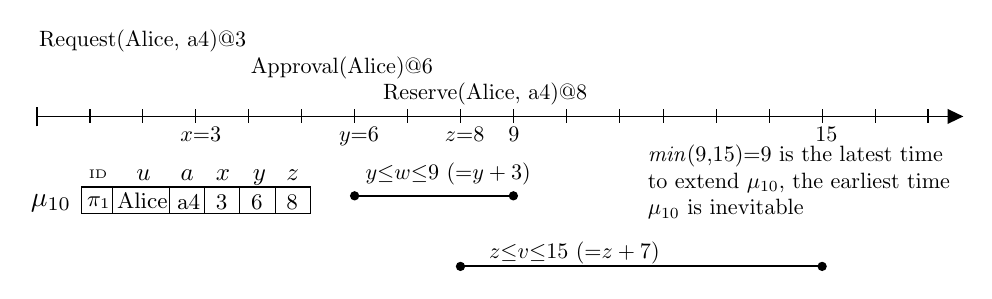
\begin{tikzpicture}[scale=0.85,x=0.75pt,y=0.75pt,yscale=-1,xscale=1]
%uncomment if require: \path (0,135); %set diagram left start at 0, and has height of 135

% Timeline
\draw    (5,35) -- (530,35) (35,31) -- (35,39)(65,31) -- (65,39)(95,31) -- (95,39)(125,31) -- (125,39)(155,31) -- (155,39)(185,31) -- (185,39)(215,31) -- (215,39)(245,31) -- (245,39)(275,31) -- (275,39)(305,31) -- (305,39)(335,31) -- (335,39)(360,31) -- (360,39)(390,31) -- (390,39)(420,31) -- (420,39)(450,31) -- (450,39)(480,31) -- (480,39)(510,31) -- (510,39)(530,31) ;
% Left End Line
\draw [shift={(5,35)}] [color={rgb, 255:red, 0; green, 0; blue, 0 }  ][line width=0.75]    (0,5.59) -- (0,-5.59)   ;
% Right Triangle
\draw [shift={(530,35)}, rotate = 180] [fill={rgb, 255:red, 0; green, 0; blue, 0 }  ][line width=0.08]  [draw opacity=0] (8.93,-4.29) -- (0,0) -- (8.93,4.29) -- cycle ;

% Timestamps Under Timeline
\draw (271,40) node [anchor=north west][inner sep=0.75pt]  [xscale=0.8,yscale=0.8] [align=left] {{9}};
\draw (445,40) node [anchor=north west][inner sep=0.75pt]  [xscale=0.8,yscale=0.8] [align=left] {{15}};

% Variables Under Timeline
\draw (85,40) node [anchor=north west][inner sep=0.75pt] [xscale=0.8,yscale=0.8] [align=left] {{$x{=}3$}};
\draw (175,40) node [anchor=north west][inner sep=0.75pt] [xscale=0.8,yscale=0.8] [align=left] {{$y{=}6$}};
\draw (235,40) node [anchor=north west][inner sep=0.75pt] [xscale=0.8,yscale=0.8] [align=left] {{$z{=}8$}};

% Assignment Boxes
\draw   (30,75) -- (48,75) -- (48,90) -- (30,90) -- cycle ;
\draw   (48,75) -- (80,75) -- (80,90) -- (48,90) -- cycle ;
\draw   (80,75) -- (100,75) -- (100,90) -- (80,90) -- cycle ;
\draw   (100,75) -- (120,75) -- (120,90) -- (100,90) -- cycle ;
\draw   (120,75) -- (140,75) -- (140,90) -- (120,90) -- cycle ;
\draw   (140,75) -- (160,75) -- (160,90) -- (140,90) -- cycle ;

% Assignment Variables
\draw (33,64) node [anchor=north west][inner sep=0.75pt][xscale=0.9,yscale=0.9] [align=left] {{\An{\tiny ID}}};
\draw (60,64) node [anchor=north west][inner sep=0.75pt][xscale=0.9,yscale=0.9] [align=left] {{$u$}};
\draw (85,64) node [anchor=north west][inner sep=0.75pt][xscale=0.9,yscale=0.9] [align=left] {{$a$}};
\draw (105,64) node [anchor=north west][inner sep=0.75pt][xscale=0.9,yscale=0.9] [align=left] {{$x$}};
\draw (126,64) node [anchor=north west][inner sep=0.75pt][xscale=0.9,yscale=0.9]  [align=left] {{$y$}};
\draw (145,64) node [anchor=north west][inner sep=0.75pt][xscale=0.9,yscale=0.9] [align=left] {{$z$}};

% Assignment Values
\draw (0,78) node [anchor=north west][inner sep=0.75pt] {$\mu_{10}$};
\draw (32,79) node [anchor=north west][inner sep=0.75pt][xscale=0.9,yscale=0.9] [align=left] {{\small $\pi_{1}$}};
\draw (49,77) node [anchor=north west][inner sep=0.75pt][xscale=0.9,yscale=0.9] [align=left] {{\small Alice}};
\draw (83,78) node [anchor=north west][inner sep=0.75pt][xscale=0.9,yscale=0.9] [align=left] {{\small a4}};
\draw (105,78) node [anchor=north west][inner sep=0.75pt][xscale=0.9,yscale=0.9]  [align=left] {{\small $3$}};
\draw (125,78) node [anchor=north west][inner sep=0.75pt][xscale=0.9,yscale=0.9]  [align=left] {{\small $6$}};
\draw (145,78) node [anchor=north west][inner sep=0.75pt][xscale=0.9,yscale=0.9] [align=left] {{\small $8$}};

% y-w Interval
\draw [line width=0.75]    (185,80) -- (275,80) ;
% Left Circle
\draw [shift={(185,80)}] [color={rgb, 255:red, 0; green, 0; blue, 0 }  ][fill={rgb, 255:red, 0; green, 0; blue, 0 }  ][line width=0.75]  (0, 0) circle [x radius= 2.0, y radius= 2.0]   ;
% Right Circle
\draw [shift={(275,80)}] [color={rgb, 255:red, 0; green, 0; blue, 0 }  ][fill={rgb, 255:red, 0; green, 0; blue, 0 }  ][line width=0.75]  (0, 0) circle [x radius= 2.0, y radius= 2.0]   ;
% y Constraint
\draw (190,60) node [anchor=north west][inner sep=0.75pt][xscale=0.8,yscale=0.8] [align=left] {{$y{\leq}w{\leq}9\ ({=}y+3)$}};

% z-v Interval
\draw [line width=0.75] (245,120) -- (450,120) ;
% Left Circle
\draw [shift={(245,120)}] [color={rgb, 255:red, 0; green, 0; blue, 0 }  ][fill={rgb, 255:red, 0; green, 0; blue, 0 }  ][line width=0.75]      (0, 0) circle [x radius= 2.0, y radius= 2.0]   ;
% Right Circle
\draw [shift={(450,120)}] [color={rgb, 255:red, 0; green, 0; blue, 0 }  ][fill={rgb, 255:red, 0; green, 0; blue, 0 }  ][line width=0.75]      (0, 0) circle [x radius= 2.0, y radius= 2.0]   ;
% z Constraint
\draw (260,105) node [anchor=north west][inner sep=0.75pt]  [xscale=0.8,yscale=0.8] [align=left] {{$z{\leq}v{\leq}15\ ({=}z+7)$}};

% Explanation Text
\draw (350,50) node [anchor=north west][inner sep=0.75pt]  [xscale=0.8,yscale=0.8] [align=left] {{\textit{min}(9,15)=9 is the latest time}\\{to extend $\mu_{10}$, the earliest time}\\{$\mu_{10}$ is inevitable}};

% Events
\draw (5,-15) node [anchor=north west][inner sep=0.75pt]  [xscale=0.8,yscale=0.8] [align=left] {{Request(Alice, a4)@3}};
\draw (125,0) node [anchor=north west][inner sep=0.75pt]  [xscale=0.8,yscale=0.8] [align=left] {{Approval(Alice)@6}};
\draw (200,15) node [anchor=north west][inner sep=0.75pt]  [xscale=0.8,yscale=0.8] [align=left] {{Reserve(Alice, a4)@8}};
%\draw (495,17) node [anchor=north west][inner sep=0.75pt]  [font=\footnotesize,xscale=0.8,yscale=0.8]  {$\pi_{1}.{\End}$};
\end{tikzpicture}
\caption{Deadline for extending potential violation, body assignment $\mu_{10}$}
\label{fig:example_deadline_minimum}
\end{figure}

Fig.\,\ref{fig:example_deadline_extension}
shows the result of a $\Payment$ event at time $9$.
This creates the assignment $\beta_2$,
leading to a new deadline calculation
for the potential extension of $\mu_{10}$
by $\beta_2$.

% \vspace*{-4mm}

\begin{figure}[h!]
  \centering

\tikzset{every picture/.style={line width=0.60pt}} %set default line width to 0.75pt        

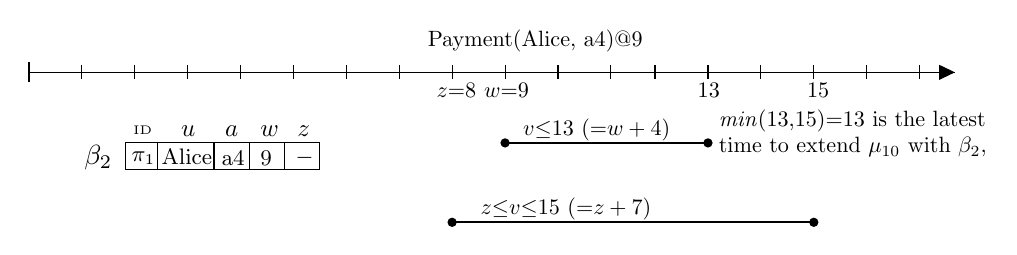
\begin{tikzpicture}[scale=0.85,x=0.75pt,y=0.75pt,yscale=-1,xscale=1]
%uncomment if require: \path (0,135); %set diagram left start at 0, and has height of 135

% Timeline
\draw    (5,35) -- (530,35) (35,31) -- (35,39)(65,31) -- (65,39)(95,31) -- (95,39)(125,31) -- (125,39)(155,31) -- (155,39)(185,31) -- (185,39)(215,31) -- (215,39)(245,31) -- (245,39)(275,31) -- (275,39)(305,31) -- (305,39)(335,31) -- (335,39)(360,31) -- (360,39)(390,31) -- (390,39)(420,31) -- (420,39)(450,31) -- (450,39)(480,31) -- (480,39)(510,31) -- (510,39)(530,31) ;
% Left End Line
\draw [shift={(5,35)}] [color={rgb, 255:red, 0; green, 0; blue, 0 }  ][line width=0.75]    (0,5.59) -- (0,-5.59)   ;
% Right Triangle
\draw [shift={(530,35)}, rotate = 180] [fill={rgb, 255:red, 0; green, 0; blue, 0 }  ][line width=0.08]  [draw opacity=0] (8.93,-4.29) -- (0,0) -- (8.93,4.29) -- cycle ;

% Timestamps Under Timeline
\draw (383,40) node [anchor=north west][inner sep=0.75pt]  [xscale=0.8,yscale=0.8] [align=left] {{13}};
\draw (445,40) node [anchor=north west][inner sep=0.75pt]  [xscale=0.8,yscale=0.8] [align=left] {{15}};

% Variables Under Timeline
\draw (235,40) node [anchor=north west][inner sep=0.75pt] [xscale=0.8,yscale=0.8] [align=left] {{$z{=}8$}};
\draw (262,40) node [anchor=north west][inner sep=0.75pt] [xscale=0.8,yscale=0.8] [align=left] {{$w{=}9$}};

% Assignment Boxes
\draw   (60,75) -- (78,75) -- (78,90) -- (60,90) -- cycle ;
\draw   (78,75) -- (110,75) -- (110,90) -- (78,90) -- cycle ;
\draw   (110,75) -- (130,75) -- (130,90) -- (110,90) -- cycle ;
\draw   (130,75) -- (150,75) -- (150,90) -- (130,90) -- cycle ;
\draw   (150,75) -- (170,75) -- (170,90) -- (150,90) -- cycle ;

% Assignment Variables
\draw (63,64) node [anchor=north west][inner sep=0.75pt][xscale=0.9,yscale=0.9] [align=left] {{\An{\tiny ID}}};
\draw (90,64) node [anchor=north west][inner sep=0.75pt][xscale=0.9,yscale=0.9] [align=left] {{$u$}};
\draw (115,64) node [anchor=north west][inner sep=0.75pt][xscale=0.9,yscale=0.9] [align=left] {{$a$}};
\draw (135,64) node [anchor=north west][inner sep=0.75pt][xscale=0.9,yscale=0.9] [align=left] {{$w$}};
\draw (156,64) node [anchor=north west][inner sep=0.75pt][xscale=0.9,yscale=0.9]  [align=left] {{$z$}};

% Assignment Values
\draw (35,75) node [anchor=north west][inner sep=0.75pt] {$\beta_{2}$};
\draw (62,79) node [anchor=north west][inner sep=0.75pt][xscale=0.9,yscale=0.9] [align=left] {{\small $\pi_{1}$}};
\draw (79,77) node [anchor=north west][inner sep=0.75pt][xscale=0.9,yscale=0.9] [align=left] {{\small Alice}};
\draw (113,78) node [anchor=north west][inner sep=0.75pt][xscale=0.9,yscale=0.9] [align=left] {{\small a4}};
\draw (135,78) node [anchor=north west][inner sep=0.75pt][xscale=0.9,yscale=0.9]  [align=left] {{\small $9$}};
\draw (155,78) node [anchor=north west][inner sep=0.75pt][xscale=0.9,yscale=0.9]  [align=left] {{\small $-$}};

% w-v Interval
\draw [line width=0.75]    (275,75) -- (390,75) ;
% Left Circle
\draw [shift={(275,75)}] [color={rgb, 255:red, 0; green, 0; blue, 0 }  ][fill={rgb, 255:red, 0; green, 0; blue, 0 }  ][line width=0.75]  (0, 0) circle [x radius= 2.0, y radius= 2.0]   ;
% Right Circle
\draw [shift={(390,75)}] [color={rgb, 255:red, 0; green, 0; blue, 0 }  ][fill={rgb, 255:red, 0; green, 0; blue, 0 }  ][line width=0.75]  (0, 0) circle [x radius= 2.0, y radius= 2.0]   ;
% y Constraint
\draw (284,60) node [anchor=north west][inner sep=0.75pt][xscale=0.8,yscale=0.8] [align=left] {{$v{\leq}13\ ({=}w+4)$}};

% z-v Interval
\draw [line width=0.75] (245,120) -- (450,120) ;
% Left Circle
\draw [shift={(245,120)}] [color={rgb, 255:red, 0; green, 0; blue, 0 }  ][fill={rgb, 255:red, 0; green, 0; blue, 0 }  ][line width=0.75]      (0, 0) circle [x radius= 2.0, y radius= 2.0]   ;
% Right Circle
\draw [shift={(450,120)}] [color={rgb, 255:red, 0; green, 0; blue, 0 }  ][fill={rgb, 255:red, 0; green, 0; blue, 0 }  ][line width=0.75]      (0, 0) circle [x radius= 2.0, y radius= 2.0]   ;
% z-v Constraint
\draw (260,105) node [anchor=north west][inner sep=0.75pt]  [xscale=0.8,yscale=0.8] [align=left] {{$z{\leq}v{\leq}15\ ({=}z+7)$}};

% Explanation Text
\draw (395,55) node [anchor=north west][inner sep=0.75pt]  [xscale=0.8,yscale=0.8] [align=left] {{\textit{min}(13,15)=13 is the latest}\\{time to extend $\mu_{10}$ with $\beta_2$,}};

% Events
\draw (230,10) node [anchor=north west][inner sep=0.75pt]  [xscale=0.8,yscale=0.8] [align=left] {{Payment(Alice, a4)@9}};
\end{tikzpicture}
\caption{Deadline for extending $\beta_2$ as match for $\mu_{10}$}
\label{fig:example_deadline_extension}
\end{figure}

With the above technical definitions
and illustration of the problem,
we can now state the main focus of this dissertation:
{\em Given a rule or a set of rules,
monitor a workflow enactment
for violations of the rule or set of rules, respectively,
as the enactment is updated with new events.}
% For more 
% We do this by calculating and updating deadlines,
% as illustrated above,
% after the arrival of each batch of events,
% along with other automated reasoning techniques.
% We then extend the approach to a set of rules
% in Section \ref{sec:multiple},
% where the consequences of rules may influence each other,
% resulting in even earlier detection
% than when rules are monitored individually.